%!TEX root = main.tex
\subsection{Introduction}
In N-Grams, each word occurence is considered as a random event.
\subsubsection{Zipf's law}

The count histogram follow the Zipf's law: $y = bx^{-a}$.

\begin{figure}[htp]
	\centering
	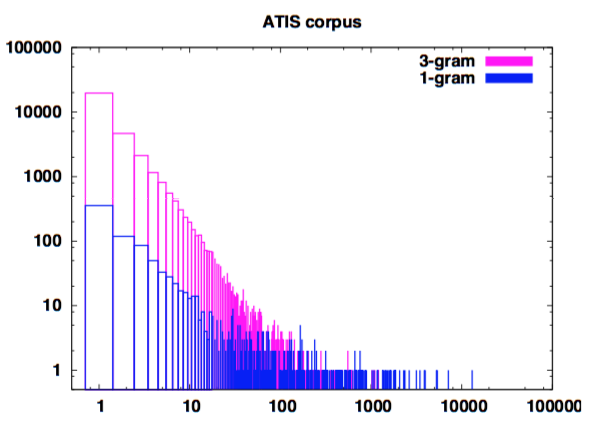
\includegraphics[scale=0.4]{images/08_zipf.png}
 	\caption{Zipf's law.}
\end{figure}

\subsubsection{N-Gram probability}

\begin{figure}[htp]
	\centering
	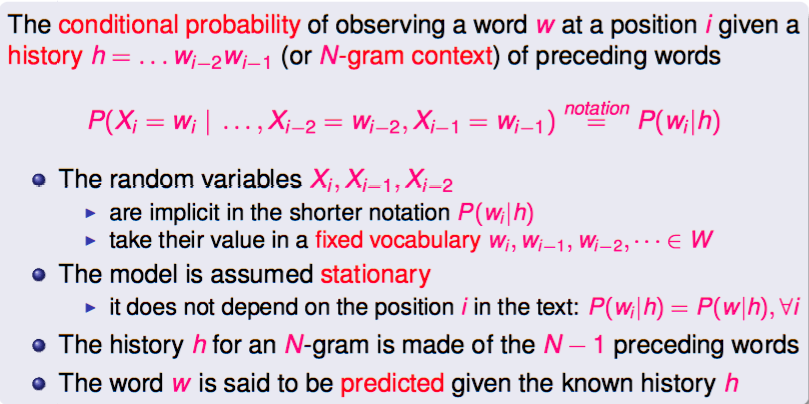
\includegraphics[scale=0.4]{images/09_proba.png}
 	\caption{N-Gram probability.}
\end{figure}

We can then compute a sentence probability if we use the chain rule and the N-Gram assumption.

\begin{figure}[htp]
	\centering
	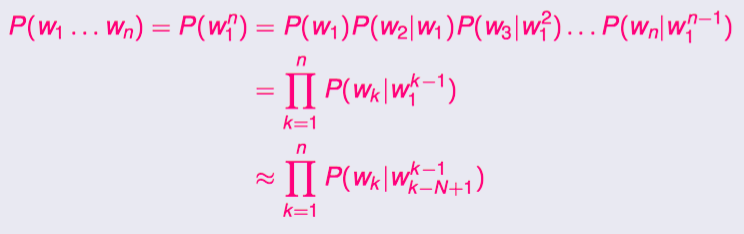
\includegraphics[scale=0.4]{images/10_sentence.png}
 	\caption{Sentence probability.}
\end{figure}

For example (3-gram): P(The rain in Spain) $\approx$ P(The) $*$ P(rain | The) $*$ P(in | The rain) $*$ P(Spain | rain in).

\subsubsection{Consistency property}

Must be verified for all models.

\begin{figure}[htp]
	\centering
	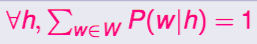
\includegraphics[scale=0.5]{images/11_consistency.png}
 	\caption{Consistency property.}
\end{figure}
\subsection{N-Gram estimation}

\subsubsection{Maximum Likelihood estimation}

\begin{figure}[htp]
	\centering
	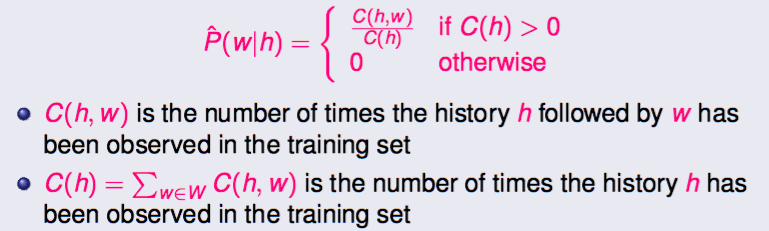
\includegraphics[scale=0.5]{images/12_likelihood.png}
 	\caption{Maximum likelihood estimation.}
\end{figure}

For unigram, $\hat{P}(w) = \frac{C(w)}{N}$ where $N$ is the size of the corpus.

\subsection{Smoothing}

Smoothing is necessary because MLE assign a zero probability to any unseen events in the training set. Many possible events are assigned a zero probability and the probability of observed events is overestimated. Smoothing techniques must respect the consistency property.

\subsubsection{Bayesian estimation}

The goal of bayesian estimation (or additive smoothing) is to add a pseudo count to avoid having probabilities of 0 for unseen events in the traning set.

\begin{figure}[htp]
	\centering
	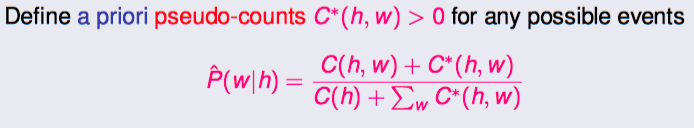
\includegraphics[scale=0.5]{images/13_bayesian.png}
 	\caption{Bayesian estimation.}
\end{figure}

The \textbf{prior probability} of the event $(h,w)$ is defined as $\frac{C^*(h,w)}{\sum_w C^*(h,w)}$. $\hat{P}(w|h)$ can be interpreted as a \textbf{posterior estimate}.

A particular form of the bayesian smoothing is the \textbf{Laplace} smoothing (or add one method).

\begin{figure}[htp]
	\centering
	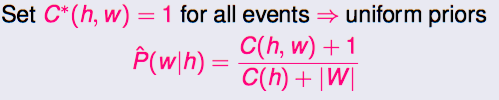
\includegraphics[scale=0.5]{images/14_add_one.png}
 	\caption{Add one method.}
\end{figure}

In general add-one smoothing is a poor method of smoothing because too much probability mass is moved to all the zeros.


\subsubsection{Linear estimation}

The goal is to build different estimators for several model orders. The differents estimators vary by history and are combined linearly.

\begin{figure}[htp]
	\centering
	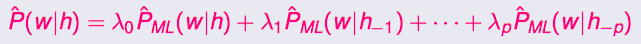
\includegraphics[scale=0.5]{images/15_linear.png}
 	\caption{Linear interpolation. $h_{-1}$: $h$ without the front word.}
\end{figure}

We need then to estimate the weights of the model: \textbf{Expectation-Maximization estimation}. The model before is a special case of the \textbf{mixture model}.

\begin{figure}[H]
	\centering
	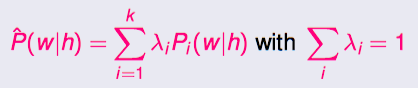
\includegraphics[scale=0.5]{images/16_mixture.png}
 	\caption{Mixture model.}
\end{figure}

We can estimate the $\lambda$'s with this algorithm:

\begin{figure}[htp]
	\centering
	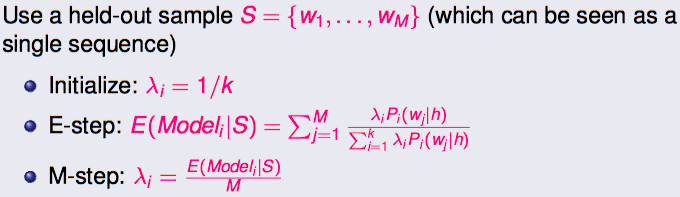
\includegraphics[scale=0.5]{images/17_em.png}
 	\caption{Expectation-Maximization algorithm.}
\end{figure}

\subsubsection{Backoff smoothing}

Idea: if we have no examples for a particular trigram, we can estimate its probability by using his bigram probability (backoff). 

\begin{figure}[H]
	\centering
	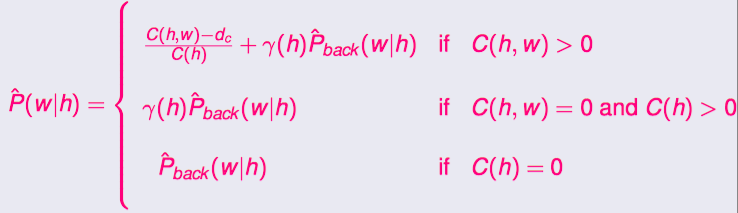
\includegraphics[scale=0.5]{images/18_backoff.png}
 	\caption{Backoff smoothing. $\hat{P}_{back}(w|h) = \hat{P}(w|h_{-1})$.}
\end{figure}

$d_c$ are the \textbf{discounting coefficients}, and $\gamma(h) = \sum_{w:C(h,w)>0} \frac{d_c}{C(h)}$.

\begin{figure}[htp]
	\centering
	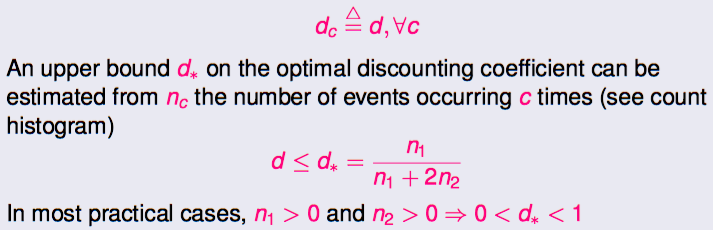
\includegraphics[scale=0.5]{images/19_discounting.png}
 	\caption{Absolute discounting.}
\end{figure}

\subsection{Performance assessment}

To test the smoothing, we can do \textbf{data splitting}:

\begin{itemize}
	\item \textbf{Basic protocol}: split data to into training (90\%, estimate the model) and test (10\%, evalute the quality of the model) files.
	\item \textbf{Refinement 1}:
	\begin{itemize}
		\item Split training set into 90\% of actual training and 10\% of held-out set (used to tune \textit{meta-parameters}: pseudo counts or $\lambda$'s and select an optimal model order)
		\item Re-train on the whole training set with any meta-parameter being fixed.
	\end{itemize}
	\item \textbf{Refinement 2}: Repeat the above using 10-fold cross validation. 
\end{itemize}

We can compute the \textbf{perplexity} too. The perplexity is a measure of quality of an iterated Shannon game.

\begin{figure}[H]
	\centering
	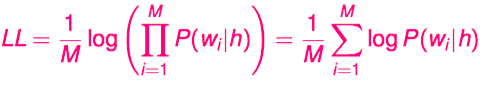
\includegraphics[scale=0.5]{images/20_log.png}
 	\caption{Per-symbol log likelihood.}
\end{figure}

\begin{figure}[H]
	\centering
	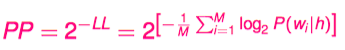
\includegraphics[scale=0.6]{images/21_perplexity.png}
 	\caption{Test set perplexity. If random (uniform) over W, $PP = |W|$. Lower the better.}
\end{figure}

If there is a word we have never see, even with a consistent and smoothed model, $P(w_{new}|h) = 0$, $PP = +\infty$. The astuce is to define a \textit{UNK} word as part of the vocabulary and relies on smoothing. 